\section{User Stories}
	\subsection{Personas}
		\begin{description}
			\item[Olivia Zander]\label{olivia}\ \newline
				\begin{minipage}[t]{0.35\textwidth} 
					\begin{figure}[H]
						\vspace{-0.75cm}
						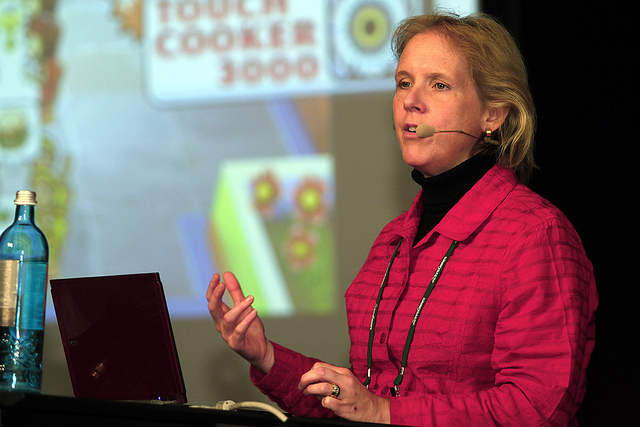
\includegraphics[trim=0cm 0cm 0cm 0cm, clip=true, width=5cm]{requirements/media/img/oliviaZander.jpg}
						\caption[Symbolbild Persona Olivia Zander\newline 
							\license{CC BY 2.0 \url{https://creativecommons.org/licenses/by/2.0/}  Official GDC \url{https://www.flickr.com/photos/officialgdc/}}
						]
						{\label{Olivia Zander}}
					\end{figure}
				\end{minipage}
				\begin{minipage}[t]{0.55\textwidth}
					52 Jahre alt.
					Olivia ist eine erfahrene \textbf{Softwarearchitektin} 
					und ist seit 14 Jahren als solche tätig.
					Zurzeit arbeitet sie in einer kleinen Beratungsunternehmung, 
					die Firmen beim Umstrukturieren von Softwareapplikationen unterstützt.
					Vor zwei Jahren absolvierte sie eine Weiterbildung im Bereich Cloud Computing.
					Seither hat sie selbst Erfahrungen mit Cloud Projekten sammeln können. 
					Sie führte verschiedene Beratungsprojekten durch, deren Ziel es war,
					bestehende Anwendungen in die Cloud zu bringen.
				\end{minipage}
			\item[Thomas Bucher]\label{thomas}\ \newline
				\begin{minipage}[t]{0.35\textwidth} 
					\begin{figure}[H]
						\vspace{-0.75cm}
						
\includegraphics[trim=0cm 0cm 0cm 0cm, clip=true, width=5cm]{requirements/media/img/thomasBucher.jpg}
						\caption[Symbolbild Persona Thomas Bucher\newline
							\license{CC BY 2.0 \url{https://creativecommons.org/licenses/by/2.0/} Steve wilson \url{https://www.flickr.com/photos/125303894@N06/}}
						]
						{\label{Thomas Bucher}}
					\end{figure}
				\end{minipage}
				\begin{minipage}[t]{0.55\textwidth}
					32 Jahre alt.
					Thomas hat vor acht Jahren in Rapperswil den Bachelor in Informatik abgeschlossen und arbeitet seither in der gleichen Firma wie Olivia.
					Er ist als \textbf{Projektplaner und technische Führungskraft} tätig und
					arbeitet je nach Projekt mit einem Team von 2-5 Entwicklern und Softwarearchitekten zusammen.
					Zurzeit unterstützt er eine externe Firma dabei,
					eine Anwendung mit täglich rund 10'000 Benutzern von ihren lokalen Servern in die Cloud zu transferieren.
				\end{minipage}
		\end{description}
		
	\subsection{Definitionen}\label{userstoryDefinitions}
		Folgende Wörter werden in den User Stories verwendet und sind zum genauen Verständnis hier definiert.
		\begin{description}			
			\item[Entscheidungswissenssverwaltung (DKS: \dks)] System, 
				das Entscheidungswissen, Entscheidungen, Optionen und getroffene Entscheidungen 
				sowie deren Abhängigkeiten speichert. Beispiel: \cdar.
			\item[Wissensproduzent] Person, die neues Wissen ins System (DKS und \eeppi)
				 einpflegt (als Beispiel kann hier \hyperref[olivia]{Olivia} dienen).
			\item[Problem Space (Wissensbaum im \cdar)] Ein Projekt in einem \dks, 
				in welchem ein Wissensproduzent Wissen ablegt.
			\item[Wissenskonsument] Person, die einen Problem Space benutzt,
				 um damit Entscheide zu fällen 
				 (als Beispiel kann hier \hyperref[thomas]{Thomas} dienen).
			\item[Solution Space (Entscheidungsprojekt im \cdar)] Ein Projekt in einem \dks, 
				aus welchem ein Wissenskonsument Wissen konsumiert.
				Ein Solution Space wird aus einem Problem Space heraus durch Kopieren erzeugt.
			\item[Administrator] Person, die für die Konfiguration 
				und den Betrieb von \eeppi\ verantwortlich ist.
			\item[Abbildung] Mit einer Abbildung lässt sich ein Datensatz 
				in einen anderen Datensatz umwandeln.
			\item[erstellen aus] Als Grundlage wird ein Datensatz genommen, 
				aus welchem ein neuer Datensatz erstellt wird.
				Anschliessend sind die beiden Datensätze voneinander unabhängig 
				und Änderungen an einem Datensatz beeinflussen den anderen Datensatz nicht.
			\item[Task] Datensatz, welcher eine Aufgabe beschreibt.
			\item[\ttpl] Datensatz, um später daraus Tasks in einem \ppt\ zu erstellen.
			% (Task-Vorlage), Entscheidungs-Vorlage: Wortwahl gemäss Duden Regel 22
			\item[Entscheidungs-Task] Task, 
				welcher zum Treffen einer Entscheidung erledigt werden muss.
				Er ist einem Problem/Solution Space Item angehängt.
			\item[Operativer Task] Task, welcher durch das Treffen einer Option entsteht.
				Er ist dementsprechend einer Option angehängt.
			\item[Problem Space Item] Datensatz, der eine Wahl mit mehreren Optionen darstellt.
				Der Datensatz ist jedoch nur eine Vorlage, 
				die Entscheidung kann noch nicht getroffen werden
			\item[Solution Space Item] Datensatz, der eine Wahl mit mehreren Optionen darstellt.
				Er wird aus einer Entscheidungs-Vorlage erstellt.
				Die Entscheidung kann jetzt getroffen werden.
			\item[Entscheid] Getroffenes (entschiedenes) Solution Space Item.
			\item[Option] Möglichkeit, wie eine Entscheidung entschieden wird.
			\item[entscheiden] Tätigkeit, 
				in welcher für ein Solution Space Item der Entscheid gefällt wird.
			\item[importieren] Anwenden einer Abbildung zur Aufnahme von Datensätzen in das \eeppi.
			\item[exportieren] Anwenden einer Abbildung zur Ausgabe von Datensätzen aus dem \eeppi.
			\item[\ppt] Externes Programm, 
				welches Tasks verwaltet und für diese Tasks eine eigene Form erwartet.
			\item[API] Schnittstelle eines Programms (sowohl bei externen, als auch bei \eeppi)
		\end{description}

		
	\begin{landscape}
	\subsection{Übersicht über die User Stories}
	
		In der folgenden Abbildung~\ref{fig:UserStoryDiagram} werden die übergeordneten User Stories beschrieben, um den ganzen Prozess vom \dks\ bis ins \ppt\ zu erfassen.
	
		\begin{figure}[H]
				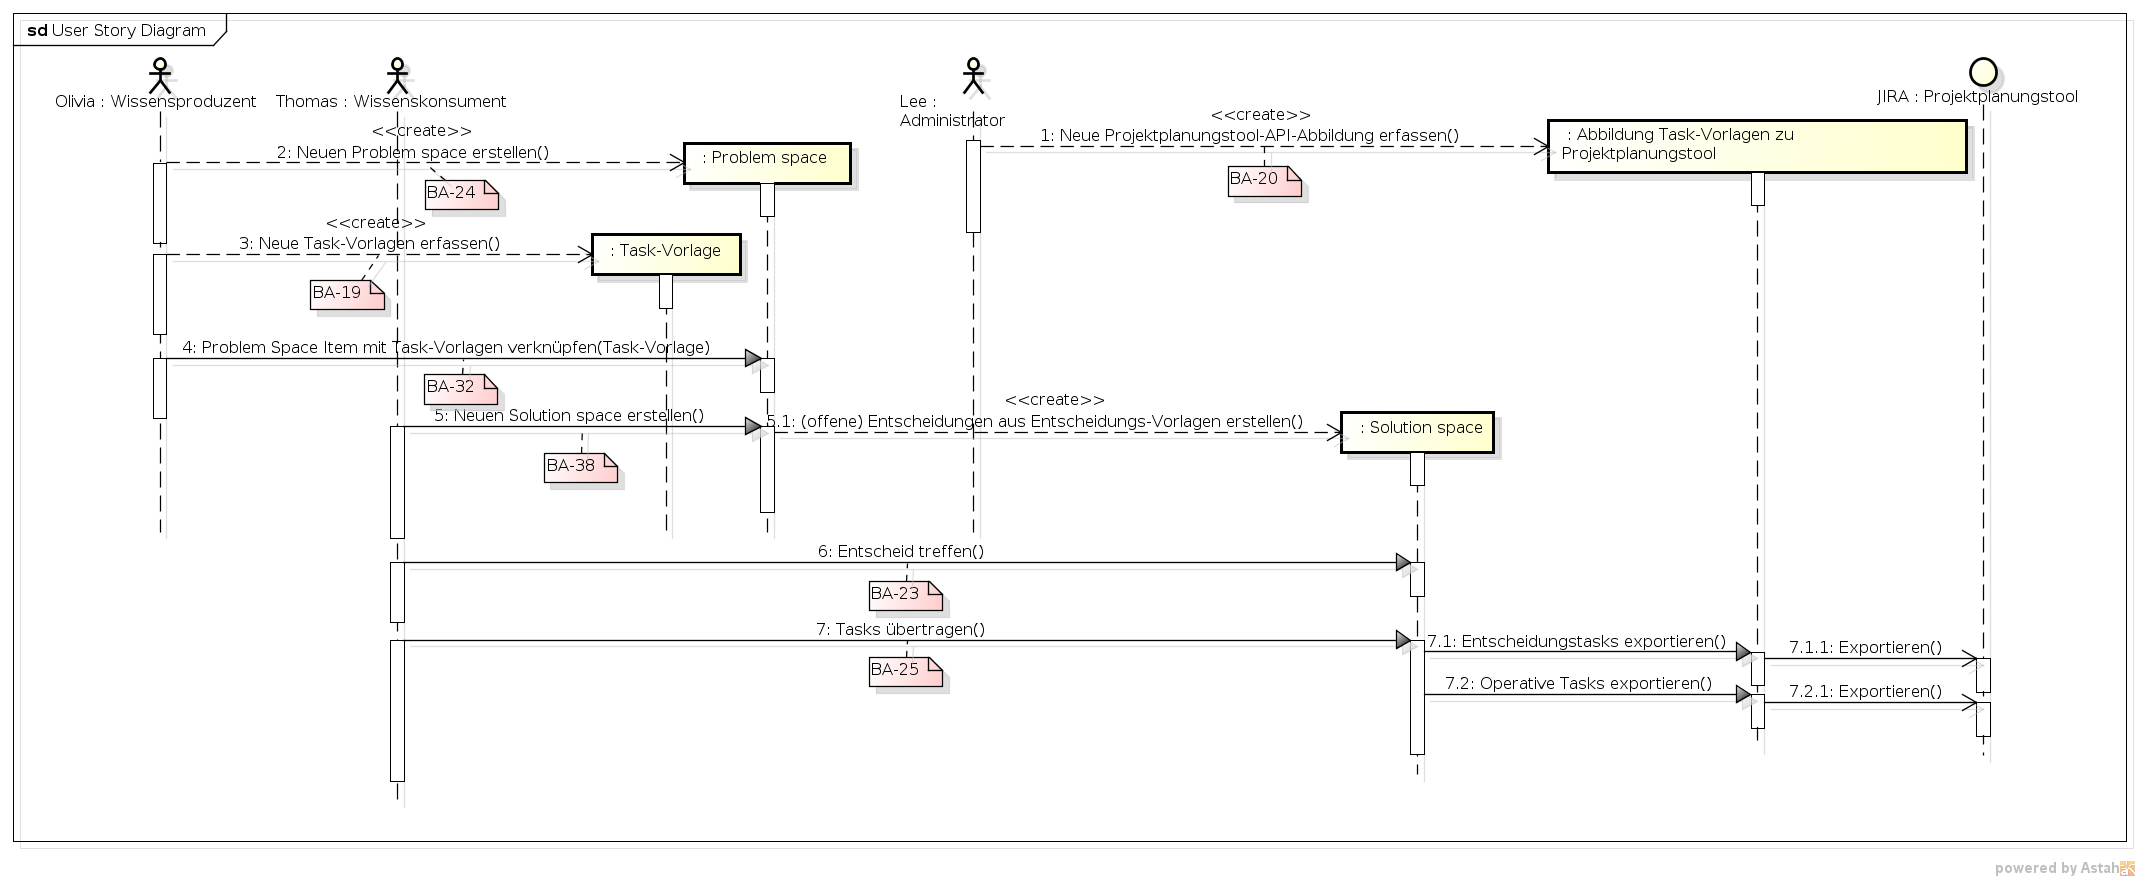
\includegraphics[width=0.95\linewidth]{media/diagrams/UserStoryDiagram.png}
				\centering
				\caption{Übergeordnete User Stories (inklusive \cdar)}
				\label{fig:UserStoryDiagram}
		\end{figure}
		
		Dabei repräsentieren die drei Aktoren (Wissensproduzent, -konsument und Administrator) Personen wie in Abschnitt~\ref{userstoryDefinitions} beschrieben,
		der Business-Aktor (ganz rechts) repräsentiert ein beliebiges \ppt\ und die roten Kästchen referenzieren den dazugehörenden Issue im \eeppi-\ppt.
		Nachfolgend sind die Erklärungen für die aufgezeigten User Stories.
		Die User Stories sind jeweils im Format nach Mike Cohn \cite{rasmusson_agile_2012} beschrieben:
		\begin{quote}
			\textbf{As a} <type of user>,\newline
			\textbf{I want} <to perform some task>\newline
			\textbf{so that I can} <achieve some goal/benefit/value>.
		\end{quote}
	\end{landscape}
	
		% http://jira.eeppi.ch/issues/?filter=10303
		% querformat, weil sonst der Text zu klein wird
		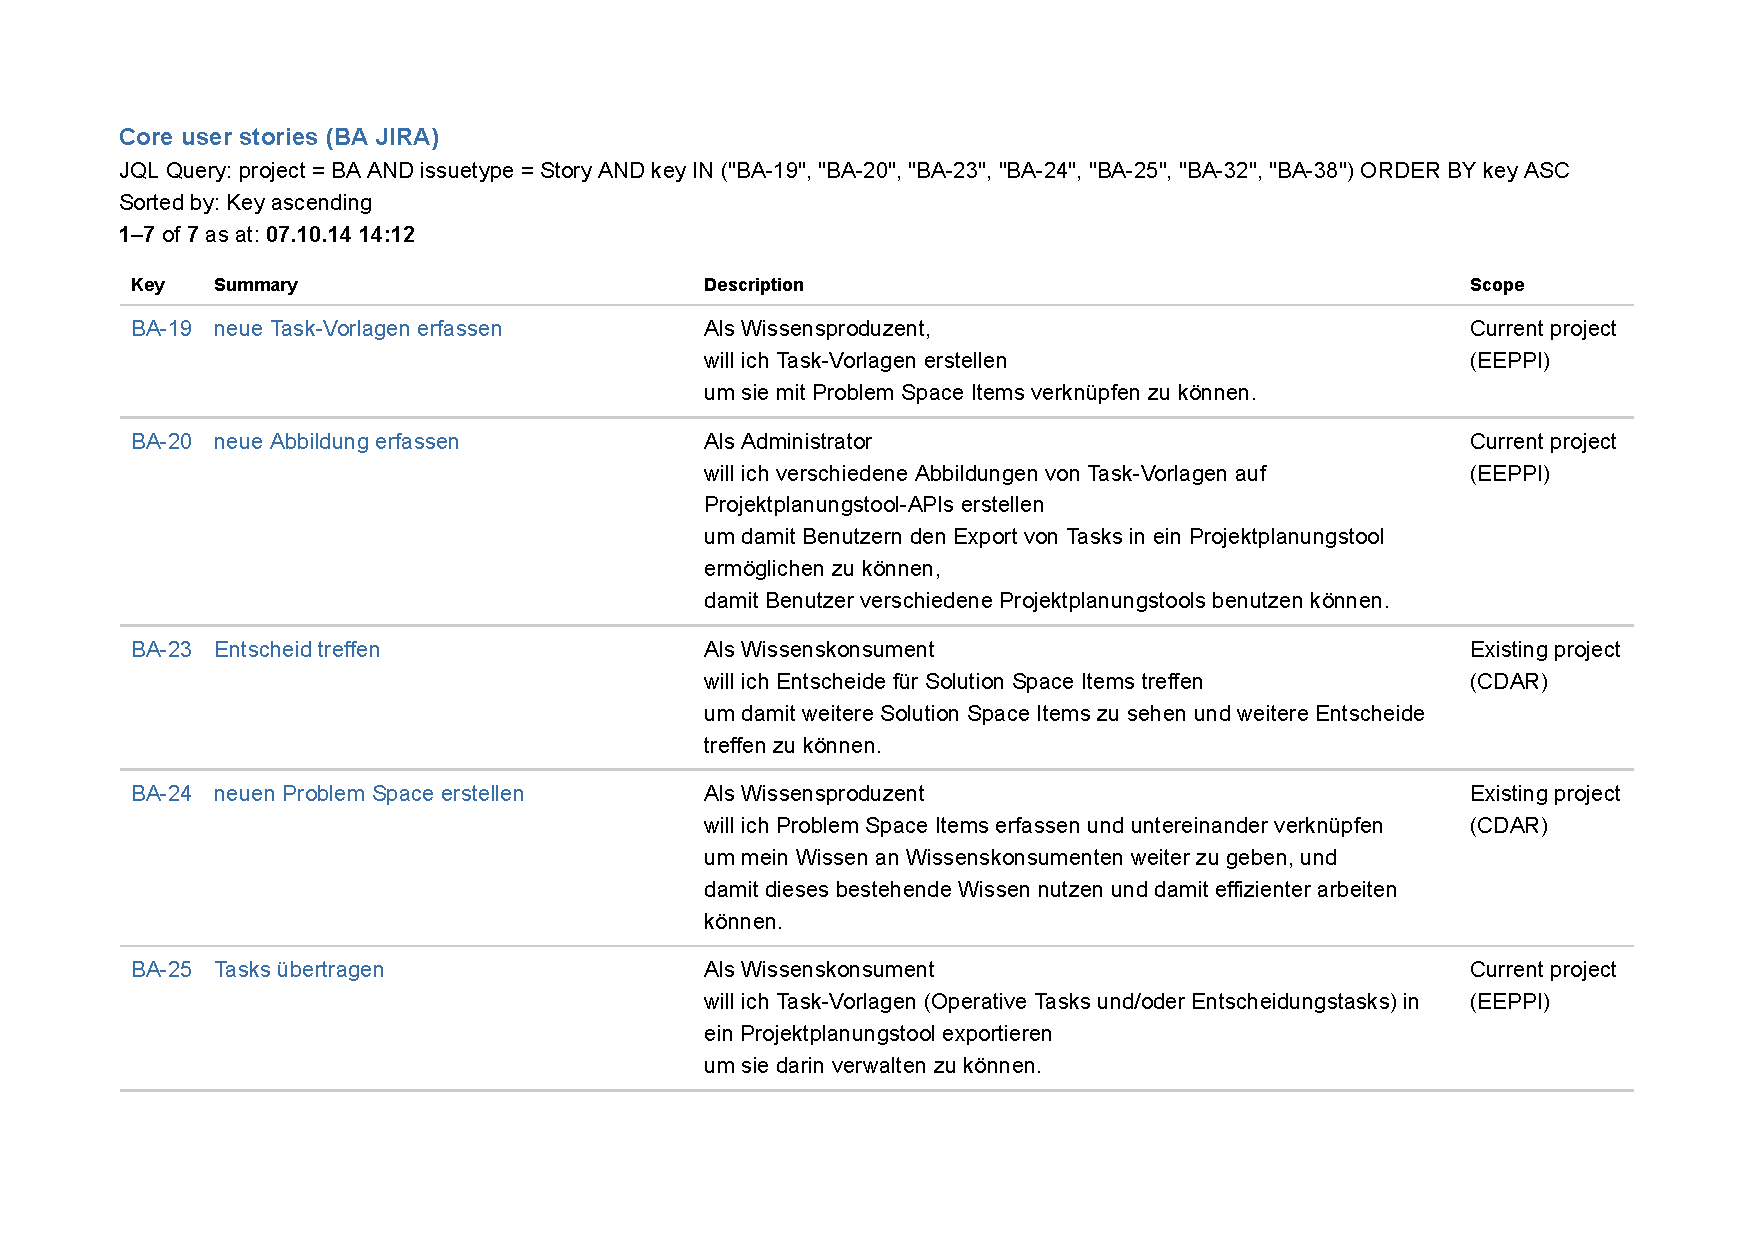
\includepdf[pages=-, pagecommand={}, scale=0.975, landscape=true]{requirements/media/documents/coreUserStories.pdf}
			
		% http://jira.eeppi.ch/issues/?filter=10304
		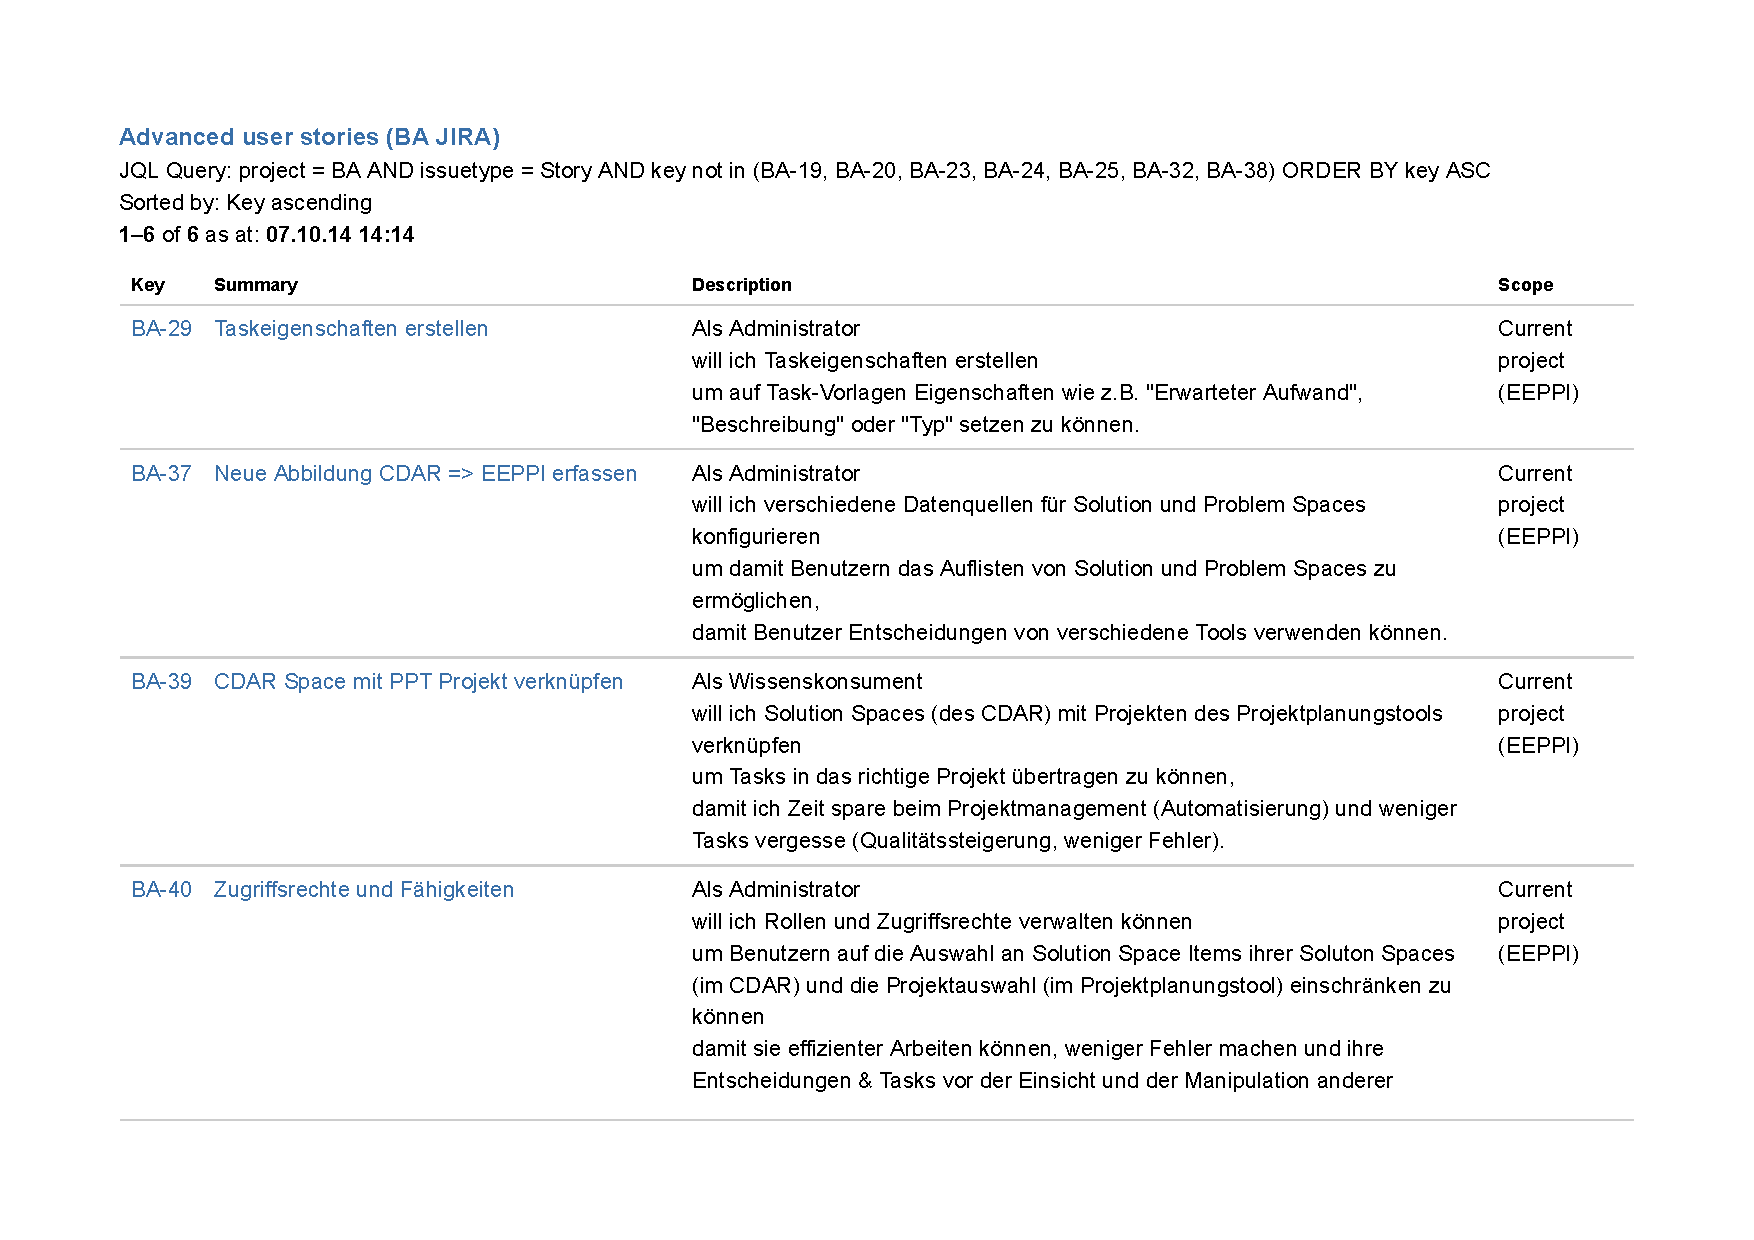
\includepdf[pages=-, pagecommand={}, scale=0.975, landscape=true]{requirements/media/documents/advancedUserStories.pdf}
			
